\chapter{Items}

Items can be Private or Shareable.
Since an Item has to belong to a Container, the Container must exist or be created first.
A Private Item can be stored in a Private or Shareable Container.
Such an Item cannot be shared with any user.
A Shareable Item can be stored only inside a Shareable Container.

\section{Create an Item}
From Main Menu bar, select "Items" tab and then select "Create new Item".
The screen with the list of Containers will show up.
To create an Item in a specific Container of interest, click on {\color{mygreen}\faPlusCircle} {\color{myblue}Add} link
on the corresponding line. You could also open the Container of interest and then click on 
{\color{mygreen}\faPlusCircle} {\color{myblue}Add} link to add an Item.

\begin{figure}[H]
\centering
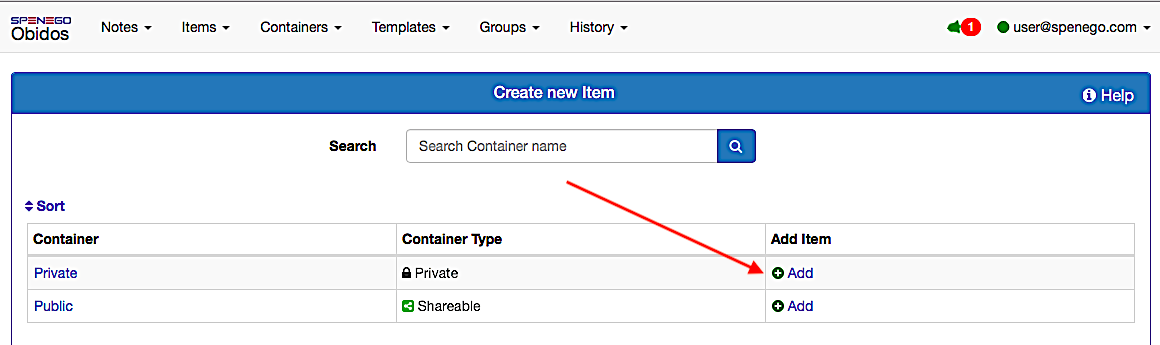
\includegraphics[width=150mm]{user/Items-Add.png}
\caption{Add an Item to a Container}
\label{fig: Figure}
\end{figure}

In the next screen it will be asked to select the type of Item. 

\begin{figure}[H]
\centering
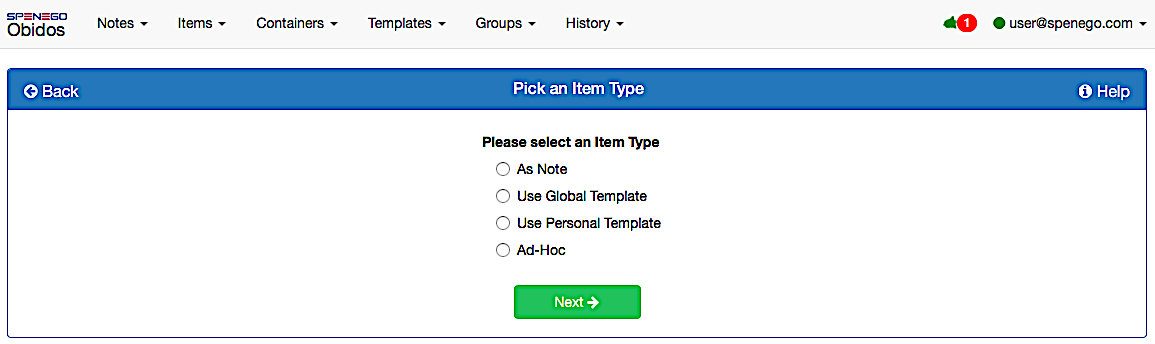
\includegraphics[width=150mm]{user/Item-Type.png}
\caption{Select the Type of the Item}
\label{fig: Figure}
\end{figure}

The Item can be created using a Global Template or Personal Template.
Or the Item can be created as a Note. It is also possible to create an ad hoc Item. An ad hoc item is a free form.
When creating a Shareable Item, it is possible to set an expiration. The user can specify the number of days after which the Item will expire. Once an Item expires, it will not be accessible.
It is not possible to set expiration on a Private Item.

\section{List Items}
Select "Items" from the Main Menu bar and then select "My Items" to set the list of all Items. Each Item will also show the Container
to which it belongs.

\begin{figure}[H]
\centering
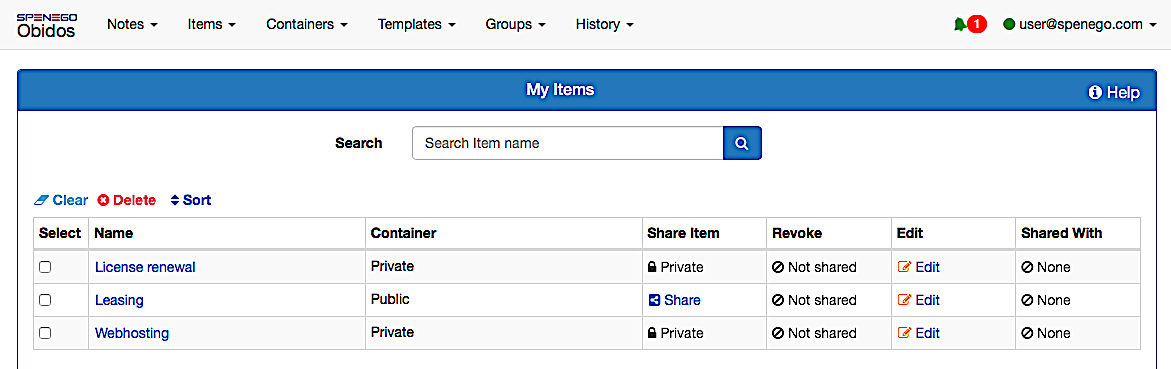
\includegraphics[width=150mm]{user/Items-List.png}
\caption{List Items in a Container}
\label{fig: Figure}
\end{figure}

%\subsection{Sorting the List of Items}
The List of Items can be sorted in alphabetical order either based on Item names or based on Container names.

\begin{figure}[H]
\centering
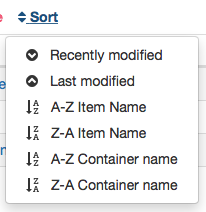
\includegraphics[scale=0.5]{user/Items-Sort.png}
\caption{Sorting Items List}
\label{fig: Figure}
\end{figure}

\section{View an Item}
Get the List of Items (see section above).
From the List of Items, on the line corresponding to the Item, click on the name of the Item of interest

\section{Edit an Item}
Get the List of Items (see section above).
From the List of Items, on the line corresponding to the Item, there will be a button to edit the Item.

\begin{figure}[H]
\centering
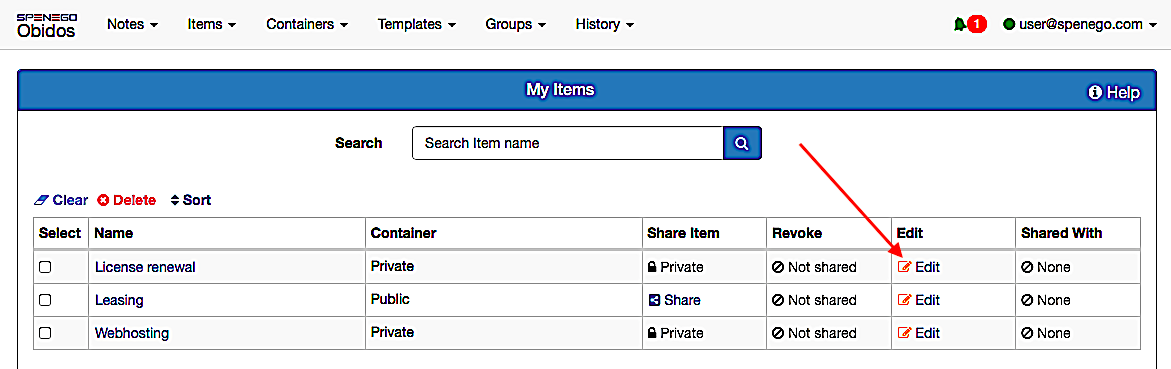
\includegraphics[width=150mm]{user/Items-Edit.png}
\caption{Edit an Item}
\label{fig: Figure}
\end{figure}

\section{Delete an Item}
Get the List of Items (see section above).
From the List of Items, select the Item(s) to delete by clicking on the button on the left of the Item(s). 
Then click on on {\color{red}\faTimesCircle \ Delete} button.

\begin{figure}[H]
\centering
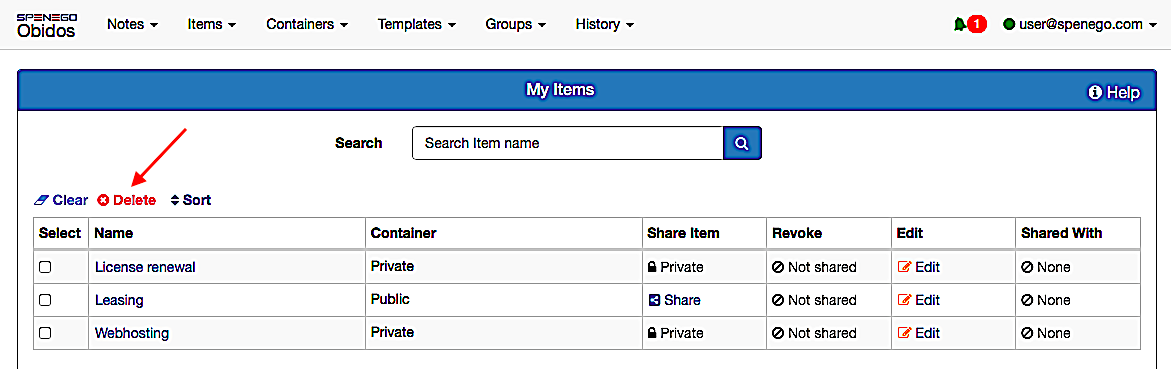
\includegraphics[width=150mm]{user/Items-Delete.png}
\caption{Deleting an Item}
\label{fig: Figure}
\end{figure}

When an Item is deleted, it will be revoked from all users to whom it was previously shared.

\section{Share an Item}
Sharing an Item can be done only from the List of Items (see section above).
From the List of Items, on the line corresponding to the Item, click on {\color{myblue}\faShareAltSquare \ Share} link
to initiate sharing of the Item.

\begin{figure}[H]
\centering
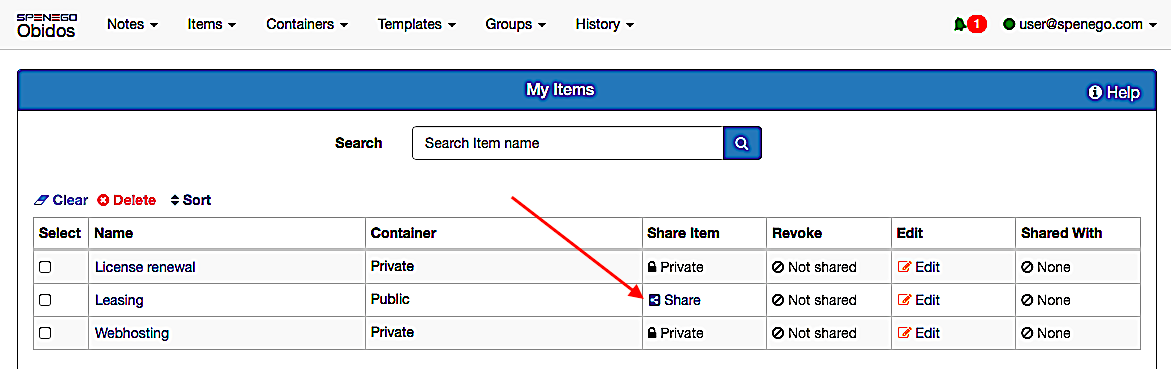
\includegraphics[width=150mm]{user/Items-Share.png}
\caption{Sharing an Item}
\label{fig: Figure}
\end{figure}

